\documentclass{standalone}
\usepackage{tikz}

\begin{document}
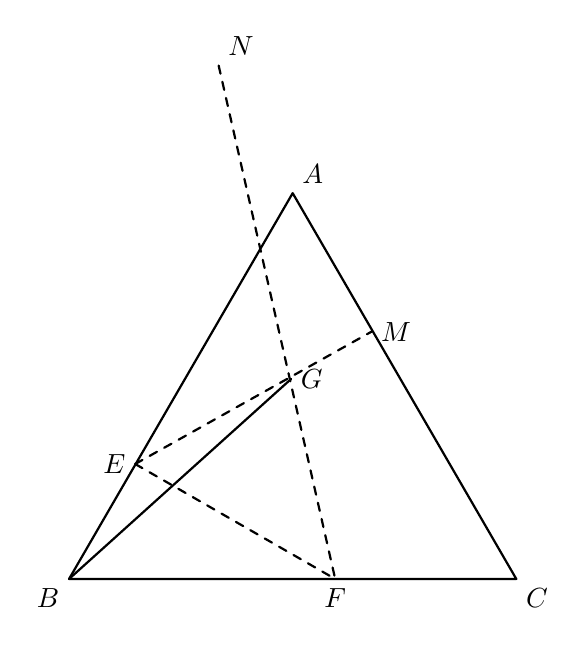
\begin{tikzpicture}[scale=1, line cap=round, line join=round]

  % 顶点与关键点坐标
  \coordinate (B) at (0,0);
  \coordinate (C) at (5.68,0);
  \coordinate (A) at (2.84,4.9);
  \coordinate (N) at (1.9,6.52);
  \coordinate (E) at (0.84,1.46);
  \coordinate (M) at (3.84,3.14);
  \coordinate (F) at (3.38,0);
  \coordinate (G) at (2.82,2.54);

  % 原有实线三角形 ABC
  \draw[thick] (B) -- (C) -- (A) -- cycle;

  % 原有虚线
  \draw[dashed, thick] (N) -- (F);
  \draw[dashed, thick] (E) -- (M);
  \draw[dashed, thick] (E) -- (F);

  % 新增实线 BG
  \draw[thick] (B) -- (G);

  % 标签
  \node[above right] at (A) {$A$};
  \node[above right] at (N) {$N$};
  \node[right] at (M) {$M$};
  \node[right] at (G) {$G$};
  \node[left] at (E) {$E$};
  \node[below] at (F) {$F$};
  \node[below left] at (B) {$B$};
  \node[below right] at (C) {$C$};

\end{tikzpicture}
\end{document}
